\documentclass{article}

\usepackage{amsthm}
	\newtheorem*{definition}{Definition}
	\newtheorem*{theorem}{Theorem}
	\newtheorem*{lemma}{Lemma}
\usepackage{amsmath}
\usepackage{amsfonts}
\usepackage{amssymb}
\usepackage[margin=1in]{geometry}
\usepackage{hyperref}
\usepackage{tikz}
	\usetikzlibrary{cd}
	\usetikzlibrary{patterns}
	
\DeclareMathOperator{\Tor}{Tor}
\DeclareMathOperator{\im}{im}
\renewcommand{\theequation}{\roman{equation}}

\title{\href{https://math.umn.edu/sites/math.umn.edu/files/exams/mantopf19.pdf}{Fall 2019 Manifolds and Topology Preliminary Exam}}
\author{University of Minnesota}
\date{}
\begin{document}
\maketitle

\section*{Part A}
\begin{enumerate}
	\item Give a precise definition of the product $\alpha * \beta$ of two paths in a space $X$, including the conditions under which it is defined.
	
	\begin{definition}
	Let $\alpha, \beta: [0,1] \rightarrow X$ be continuous functions into $X$. If $\alpha (1) = \beta(0)$, then the product
	$\alpha * \beta: [0,1] \rightarrow X$ is defined to be 
	\[ (\alpha * \beta ) (t) = \begin{cases} \alpha(2t) & t \in [0,1/2] \\  \beta(2t-1) & t \in (1/2,1]\end{cases}\].
	\end{definition}
	
	\item Suppose that $X$ is a path connected, semilocally 1-connected space whose fundamental group is $\mathbb{Z}/2 \times \mathbb{Z}/2$. How many isomorphism classes of connected covering spaces does $X$ have?
	
	% See Hatcher prop 1.38
	\begin{proof}
		The isomorphism classes of covering spaces correspond to conjugacy classes of the fundamental group. 
		Thus, this question is equivalent to counting the conjugacy classes of $\mathbb{Z}/2 \times \mathbb{Z}/2$.
		Note that $\mathbb{Z}/2 \times \mathbb{Z}$ is abelian and abelian groups have exactly one conjugacy class for each group element (since $h g h^{-1} = h h^{-1} g = g$ for any $g,h$).
		Thus, there are $|\mathbb{Z}/2 \times \mathbb{Z}/2| = 4$ conjugacy classes, and hence there are $4$ isomorphism classes of covering spaces of $X$.
	\end{proof}
	
	\item Give an example of a space $X$ with open subsets $U,V$ such that $X = U\cup V$, $U$ is simply connected, $V$ is simply connected, but where $X$ is not simply connected. 
	Then explain why this does not violate the Siefert-van Kampen theorem. 
	
	\begin{proof}
		Let $X$ be the annulus of inner radius $1$ and outer radius $2$, shown below,:
		
		\begin{center}
			% TODO: Make this picture prettier.
                    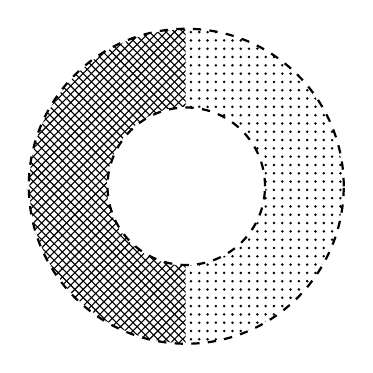
\begin{tikzpicture}
                    	\filldraw[pattern=dots,draw=white] (0 ,-1) arc [radius=1, start angle=-90, delta angle=180]
                  				-- (0,2) arc [radius=2, start angle=90, delta angle=-180]
                 				 -- cycle;
				 
			\filldraw[pattern=crosshatch, draw=white] 
						(0,1) arc [radius=1, start angle=90, delta angle=180]
                  				-- (0,-2) arc [radius=2, start angle=-90, delta angle=-180]
                 				 -- cycle;
				 
			%\draw[thick] (0,1) -- (0,2);
			%\draw[thick] (0,-1) -- (0,-2);
                    	\draw[thick, dashed] (0,0) circle (2cm);
			\draw[thick, dashed] (0,0) circle (1cm);
		
                    \end{tikzpicture}
                    \end{center}
                    
                    and let $U$ be the left half of the annulus (shown crosshatched) with $\epsilon$ extra and let $V$ be the right half of the annulus (shown filled with dots) also with $\epsilon$ extra, where both $U, V$ intersect in $\epsilon$-fattenings of the line segments $\ell_+ = [(0,1),(0,2)]$ and $\ell_-=[(0,-1),(0,-2)]$.
                    
                    Then $\pi_1(U) = \pi_1(V) = 0$ since both are contractible. Additionally, $\pi_1(U \cap V) =  0$ since both the $\epsilon$-fattenings of line segments $\ell_+, \ell_-$ are contractible so regardless of choice of basepoint we are in a contractible connected component. $U$ and $V$ do not violate the hypothesis of the Siefert-van Kampen theorem, because the intersection $U \cap V$ is not path-connected. However if we were to ignore the requirement of path-connectedness, we might conclude that the theorem says $\pi_1(X) = 0/0 \cong 0$.
                    
                    But we know that $\pi_1( U \cup V) \cong \mathbb{Z}$ because the generators are the trivial loop and the loop which contains the hole in its interior.
                    
                    Thus, we cannot choose $U,V$ as in this example if we wish to use the Siefert-van Kampen theorem.
	\end{proof}
	
	\item Explain why the inclusion $\mathbb{R}^2 \backslash \{0\} \rightarrow \mathbb{R}$ is not a covering map.
	
	% See Hatcher prop 1.31
	\begin{proof}
		Suppose $\iota : \mathbb{R}^2 \backslash \{ 0 \} \rightarrow \mathbb{R}$ were a covering map. 
		
		Then it is a theorem that the induced map on fundamental groups $\iota_*: \pi_1(\mathbb{R}^2 \backslash \{ 0 \}) \rightarrow \pi_1(\mathbb{R})$ is an injection. 
		
		On the other hand, $\pi_1 (\mathbb{R}^2 \backslash \{ 0 \}) \cong \mathbb{Z}$ and $\pi_1( \mathbb{R} ) = 0$ and so no injection from $\mathbb{Z} \rightarrow 0$ exists, contradicting that $\iota$ were a covering map.
	\end{proof} 
	
	\item Define the \textit{degree} of a map $f: S^n \rightarrow S^n$ for $n > 0$. Explain why $n=0$ is a special case.
	
	\begin{definition}
		Let $n>0$ and $f: S^n \rightarrow S^n$ be a map. Then there is an induced homomorphism on homology $f_* : H_n (S^n) \rightarrow H_n (S^n)$. Since $H_n(S^n) \cong \mathbb{Z}$, then $f_*$ must be multiplication by an integer (otherwise it would not be a homomorphism). The integer $k$ such that $f_*(x) = kx$ is called the degree of the map.
		
		Note that $n=0$ is a special case, since $H_0(S^0) \cong \mathbb{Z}^2$, and so ``multiplication by an integer" must be more carefully defined.
	\end{definition}
	
	\item Suppose $X, Y$ are spaces that are both abstractly homeomorphic to $S^7$. Show that the ``degree" of the map $f: X \rightarrow Y$ is only well-defined up to sign.
	
	\item Let $X$ be the space of upper triangular invertible $2\times 2$ matrices:
	\[X = \left \{ \begin{bmatrix} a & b \\ 0 & d \end{bmatrix} \in M_2 (\mathbb{R}) : a \neq 0, d \neq 0\right \} \subseteq \mathbb{R}^3\]
	 Determine the homology groups $H_*(X)$. 

	%See Hatcher section 3.B
	
	\begin{proof}
		First, note that $X \cong (\mathbb{R} \backslash \{0\}) \times (\mathbb{R}) \times (\mathbb{R} \backslash \{0\})\subseteq \mathbb{R}^3$ by the map taking $\begin{bmatrix} a & b \\ 0 & d \end{bmatrix} \mapsto (a,b,d)$.
		
		Thus, we compute the homology groups $H_*(\mathbb{R} \backslash \{0\})$ and $H_*(\mathbb{R})$.
		
		Since $X_1 := \mathbb{R} \backslash \{0\}$ is the disjoint union of the strictly positive real axis $\mathbb{R}_{> 0}$ and the strictly negative real axis $\mathbb{R}_{< 0}$, which are homeomorphic via the map $x \mapsto -x$,
		we have 
		\[H_n(\mathbb{R}_{> 0}) = H_n(\mathbb{R}_{< 0}) = \begin{cases} \mathbb{Z} &n=0 \\ 0 &\text{else}  \end{cases} \]
		Which means that
		\[H_n(\mathbb{R} \backslash 0) = H_n(\mathbb{R}_{< 0}\sqcup \mathbb{R}_{> 0} ) = H_n(\mathbb{R}_{< 0}) \oplus H_n(\mathbb{R}_{> 0} )  = \begin{cases} \mathbb{Z}^2 & n=0 \\ 0 & \text{else} \end{cases}\]
		
		%NEED SOME EXPOSITION HERE.
		
		For CW-complexes $A,B$ a K\"unneth formula tells us that the following is a short exact sequence:
		\begin{equation} 0 \rightarrow \bigoplus_i \left ( H_i(A) \otimes H_{n-i}(B) \right ) \rightarrow H_n(A\times B) \rightarrow
		\bigoplus_i \Tor \left ( H_i(A), H_{n-i-1}(B) \right ) \rightarrow 0 \label{seq:Kunneth}\end{equation}
		
		We will first compute $H_\bullet (\mathbb{R} \times \mathbb{R}\backslash 0)$, taking $\mathbb{R} = A$ and $\mathbb{R}\backslash 0 = B$.
		
		Rewriting the above sequence for our case, we see 
		\[ 0 \rightarrow \bigoplus_i \left ( H_i(\mathbb{R}) \otimes H_{n-i}(\mathbb{R}\backslash 0) \right ) \rightarrow H_n(\mathbb{R}\times \mathbb{R}\backslash 0) \rightarrow
		\bigoplus_i \Tor \left ( H_i(\mathbb{R}), H_{n-i-1}(\mathbb{R}\backslash 0) \right ) \rightarrow 0\]
		
		First, note that for every $i$ we have $H_i(\mathbb{R})$ is torsion-free, so $\Tor \left ( H_i(\mathbb{R}), H_{n-i-1}(\mathbb{R}\backslash 0) \right ) = 0$, hence
		\[ \bigoplus_i \left ( H_i(\mathbb{R}) \otimes H_{n-i}(\mathbb{R}\backslash 0) \right ) \cong H_n(\mathbb{R}\times \mathbb{R}\backslash 0) \]
		
		When $n =0$ we have 
		\[H_0 (\mathbb{R}) \otimes H_0 (\mathbb{R} \backslash 0) = \mathbb{Z} \otimes \mathbb{Z}^2 \cong \mathbb{Z}^2\]
		
		When $n>0$ we have 
		\[ H_i(\mathbb{R}) \otimes H_{n-i}(\mathbb{R}\backslash 0) = \left (\begin{cases} 
			\mathbb{Z} \otimes 0 & i=0\\  
			0 \otimes 0 & i \neq 0,n\\
			0 \otimes \mathbb{Z}^2 & i = n\\
			\end{cases} \right) = 0 ,\]
		and so
		\[H_{n}( \mathbb{R} \times \mathbb{R}\backslash 0) = \begin{cases} \mathbb{Z}^2 & n=0 \\ 0 &\text{else} \end{cases}.\]
		
		We now use (\ref{seq:Kunneth}) with $A = \mathbb{R} \backslash 0$ and $B = \mathbb{R} \times \mathbb{R} \backslash 0$ and the fact that every homology group of $A$ is torsion-free to see
		\[ \bigoplus_i \left ( H_i(\mathbb{R} \backslash 0) \otimes H_{n-i}(\mathbb{R} \times \mathbb{R}\backslash 0) \right ) \cong H_n(\mathbb{R} \backslash 0 \times\mathbb{R}\times \mathbb{R}\backslash 0) \cong H_n(X).\]
		
		Arguing as above we see when $n=0$ that
		\[ H_0(\mathbb{R} \backslash 0) \otimes H_0(\mathbb{R} \times \mathbb{R}\backslash 0) = \mathbb{Z}^2 \otimes \mathbb{Z}^2 \cong \mathbb{Z}^4,\]
		and 
		for $n >0$ 
		\[ H_i(\mathbb{R} \backslash 0 ) \otimes H_{n-i}(\mathbb{R} \times \mathbb{R}\backslash 0) = \left (\begin{cases} 
			\mathbb{Z}^2 \otimes 0 & i=0\\  
			0 \otimes 0 & i \neq 0,n\\
			0 \otimes \mathbb{Z}^2 & i = n\\
			\end{cases} \right) = 0 ,\]
		and so 
		\[ H_n(X) = \begin{cases} \mathbb{Z}^4 & n=0 \\ 0 & \text{else} \end{cases}\]
	\end{proof}
	
	
\item Suppose $X$ is a space with open subsets $U,V$ such that $X = U \cup V$ and both $U$ and $V$ are contractable. What is the relationship between the homology groups of $X$ and $U\cap V$

\begin{proof}
The Mayer-Vietoris sequence tells us that the following sequence is exact:

\begin{tikzcd}
\cdots \arrow{r} & \tilde{H}_{n} (U \cap V) \arrow{r} & \tilde{H}_n(U) \oplus \tilde{H}_n(V) \arrow{r} & \tilde{H}_n (U \cup V) \arrow{r} &\tilde{H}_{n-1} (U \cap V) \arrow{r} & \cdots
\end{tikzcd}

Since $U,V$ are contractable, $\tilde{H}_n(U) = \tilde{H}_n(V) = 0$ for all $n$. Thus, we have the exactness of the sequence

\begin{center}
\begin{tikzcd}
\cdots \arrow{r} & 0 \arrow{r} & \tilde{H}_n (U \cup V) \arrow{r} &\tilde{H}_{n-1} (U \cap V) \arrow{r} & 0 \arrow{r} & \cdots
\end{tikzcd} \end{center}

and so we have that $\tilde{H}_n (X) \cong \tilde{H}_{n-1}(U \cap V)$ for all $n$. 

\end{proof}

\item Suppose that $X$ is a path connected space, $A$ is a path connected subspace, $p \in A$, and $C$ is the mapping cone
\[ \left ( X \times \{1\} \cup A \times [0 ,1 ] \right ) / \{ (a,0) \sim (a^\prime,0) \}. \]
Use the Seifert-Van Kampen theorem to express the fundamental group $\pi_1 (C, [(p, 1/2)])$ in terms of the map $\pi_1 (A,p) \rightarrow \pi_1(X,p)$.

\begin{proof}
The Seifert-Van Kampen theorem tells us the following commutative diagram:
\begin{center}
\begin{tikzcd}
& \pi_1(X \times \{1\} ) \arrow[dr,"\Phi"] & \\
\pi_1(A \times \{1\} ) \arrow[ur] \arrow[dr]& & \pi_1(C) \\
& \pi_1(A \times [0,1] / \{ (a,0) \sim (a^\prime, 0)\} ) \arrow[ur] &
\end{tikzcd}
\end{center}
and in particular that $\Phi$ is surjective.

Noether's first isomorphism theorem tells us that $ \pi_1(C) = \im \Phi \cong \pi_1(X)/\ker \Phi.$
Since $A \times [0,1] / \sim$ is contractable (e.g. onto the point $(a,0)$) we know that $\pi_1(A\times \{1\})$ 
is contained in the kernel of $\pi_1(X)$.
On the other hand, the surjection $\Phi$ is constructed by a quotient of the free product $\pi_1(X\times \{1\}) * 0$
by the normal subgroup generated by loops in $\pi_1(A\times\{1\})$, and so the kernel contains \emph{only} 
points in $\pi_1(A \times \{1\})$. Thus, $\pi_1(C) \cong \pi_1(X \times \{1\})/\pi_1(A \times \{1 \}) \cong \pi_1(X)/\pi_1(A)$.

Strictly speaking, we have computed $\pi_1(C,(p,1))$. However, since everything we have dealt with is path connected,
we obtain the isomorphism $\pi_1(C, (p,1)) \cong \pi_1(C, (p, 1/2))$. 

\end{proof}
	
\setcounter{enumi}{9}
\item State the \emph{unique path lifting} theorem for covering maps.\footnote{I think they are asking for thm. 1.34 of Hatcher, but I am not 100\% sure.}

\begin{theorem}
Let $p: \tilde{X} \rightarrow X$ be a covering map, and let $\gamma: [0,1] \rightarrow X$ be a
path in $X$. Let $\gamma_1: [0,1] \rightarrow \tilde{X}$ and $\gamma_2: [0,1]\rightarrow \tilde{X}$
be two lifts of $\gamma$. If there is any $t_0 \in [0,1]$ such that $\gamma_1(t_0) = \gamma_2(t_0)$, then
$\gamma_1(t) = \gamma_2(t)$ for all $t \in [0,1]$.
\end{theorem}

\end{enumerate}

\section*{Part B}
\begin{enumerate}
	\item Give an example of a compact $2$-dimensional manifold $M$ for which there exists an embedding of $M \rightarrow \mathbb{R}^n$ into Euclidean space of strictly smaller dimension than that given by the Whitney embedding theorem.
	
	\begin{proof}
		The Whitney embedding theorem states that a $d$-dimensional manifold with or without boundary can be properly smoothly embedded in $\mathbb{R}^{2d+1}$. Here, we take $d=2$ and so the embedding certainly exists in $\mathbb{R}^5$.
		
		Consider the subset of $\mathbb{R}^2$ given by $I^2:=[0,1]\times [0,1]$. 
		As a closed and bounded subset of $\mathbb{R}^2$ the Heine-Borel theorem tells us this is certainly compact. 
		
		Now consider the map $f: \mathbb{R}^2 \rightarrow \mathbb{R}^3$ taking $(x,y) \mapsto (x,y,0)$. 
		This is a smooth, proper embedding of $I^2$ into $\mathbb{R}^3$ a Euclidean space of dimension strictly smaller than $5$.
		To see that the map is smooth, note that $\frac{\partial f}{\partial x} = \frac{\partial f}{\partial y} = 1$ and $\frac{\partial f}{\partial z} = 0$.
		%% Does this hit all the requirements of proof? I'm not sure -tk
	\end{proof}
	
	
	\item The cylindrical coordinate change is given by \[(x,y) = ( r \cos (\theta), r \sin (\theta)).\]
	Express the vector field \[(x^2+y^2)^{-2/3} \left ( x \frac{\partial}{\partial x} + y \frac{\partial}{\partial y} \right) \]
	in $(r,\theta)$ coordinates.
	
	% For further details see Lee Intro to smooth manifolds, example 3.16, pg. 64
	
	\begin{proof}

		
		Now recall that the change of coordinate map $F$ which sends $(x,y)$ coordinates to $(r, \theta)$ coordinates are $r = \sqrt{x^2+y^2}$ and $\theta = \arctan(\frac{y}{x})$, and so
		\begin{align*}
			\frac{\partial r}{\partial x} &= \frac{1}{2 \sqrt{x^2+y^2}} \frac{\partial (x^2+y^2)}{\partial x}\\
			&= \frac{1}{2 \sqrt{x^2+y^2}} (2x) \\
			&= \frac{x}{ \sqrt{x^2+y^2}} \\
		\end{align*}
		and by symmetry $\frac{\partial r}{\partial y} = \frac{y}{ \sqrt{x^2+y^2}} $.
		%
		Now we compute $\frac{\partial \theta}{\partial x}$ and $\frac{\partial \theta}{ \partial y}$.
		First,
		\begin{align*}
			\frac{\partial \theta}{\partial x} &= \frac{1}{1+(y/x)^2}\frac{\partial (y/x)}{\partial x} \\
			&=\frac{1}{1+(y/x)^2} \cdot \frac{-y}{x^2}\\
			&=\frac{-y}{x^2+y^2}.
		\end{align*}
		Next,
		\begin{align*}
			\frac{\partial \theta}{\partial y} &= \frac{1}{1+(y/x)^2}\frac{\partial (y/x)}{\partial y} \\
			&=\frac{1}{1+(y/x)^2} \cdot \frac{1}{x}\\
			&=\frac{1}{1+(y/x)^2} \cdot \frac{x}{x^2}\\
			&=\frac{x}{x^2+y^2}. 		
		\end{align*}
%
		The chain rule tells us that
		%
		\begin{align*}
			 \frac{\partial}{\partial x} &= \frac{\partial }{\partial r} \frac{\partial r}{\partial x} + \frac{\partial }{\partial \theta} \frac{\partial \theta}{\partial x}  \\
			 &= \frac{x}{\sqrt{x^2+y^2}} \frac{\partial }{\partial r}  - \frac{y}{x^2+y^2}\frac{\partial }{\partial \theta}\\
			 &= \cos \theta  \frac{\partial }{\partial r}  - \frac{\sin \theta}{r}\frac{\partial }{\partial \theta}\\
		\end{align*}
		and
		\begin{align*}
			 \frac{\partial}{\partial y} &= \frac{\partial }{\partial r} \frac{\partial r}{\partial y} + \frac{\partial }{\partial \theta} \frac{\partial \theta}{\partial y} \\
			 &=  \frac{y}{\sqrt{x^2+y^2}}\frac{\partial }{\partial r}  + \frac{x}{x^2+y^2}\frac{\partial }{\partial \theta}\\
			 &= \sin \theta \frac{\partial}{\partial r} + \frac{\cos \theta}{r} \frac{\partial}{\partial \theta}
		\end{align*}
		
		Finally, we change coordinates on $x,y$, leaving their differentials unchanged, then we substitute using the expressions for $\partial/ \partial x$ and $\partial/ \partial y$ which we found above and reduce using the Pythagorean trigonometric identity to see that the vector field in terms of cylindrical coordinates is:
%		
		\begin{align*}
			(x^2+y^2)^{-2/3} \left ( x \frac{\partial}{\partial x} + y \frac{\partial}{\partial y} \right) 
			&=  ((r \cos \theta)^2+(r \sin \theta)^2)^{-2/3} \left ( (r \cos \theta) \frac{\partial}{\partial x} + (r \sin \theta) \frac{\partial}{\partial y} \right) \\
			&= r^{-4/3} \left ( (r \cos \theta) \frac{\partial}{\partial x} + (r \sin \theta) \frac{\partial}{\partial y} \right) \\
			&=  r^{-4/3} \left ( (r \cos \theta)\left(\cos \theta  \frac{\partial }{\partial r}  - \frac{\sin \theta}{r}\frac{\partial }{\partial \theta} \right) + (r \sin \theta)\left ( \sin \theta \frac{\partial}{\partial r} + \frac{\cos \theta}{r} \frac{\partial}{\partial \theta} \right ) \right) \\
			&= r^{-4/3} \left ( (r \cos^2 \theta + r \sin^2 \theta) \frac{\partial}{\partial r} + ( - \sin \theta \cos \theta + \cos \theta \sin \theta ) \frac{\partial}{\partial \theta} \right) \\
			&= r^{-4/3} \left ( r \frac{\partial}{\partial r}  \right)\\
			&= \frac{1}{\sqrt[3]{r}} \frac{\partial}{\partial r} 
			\end{align*}
	\end{proof}
	
	\item Determine the Lie bracket of the vector fields $x \frac{\partial}{\partial x} + y \frac{\partial}{\partial y}$ and $y \frac{\partial}{\partial x} - x \frac{\partial}{\partial y}$ on $\mathbb{R}^2$.
	
	% See Lee pg. 185
	
	\begin{proof}
		If $M$ is a smooth manifold with or without boundary and 
		$X = X^i \frac{\partial}{\partial x^i}$ and $Y = Y^j \frac{\partial}{\partial x^j}$
		are vector fields, then the Lie bracket is 
		\[ [X,Y] = \left ( X^i \frac{\partial Y^j}{\partial x^i} - Y^i \frac{ \partial X^j}{\partial x^i} \right ) \frac{\partial }{\partial x^j}.\]
		
		Since we are working in $\mathbb{R}^2$, then $x^1 =x$ and $x^2=y$. Define $X:= x \frac{\partial}{\partial x} + y \frac{\partial}{\partial y}$
		so $X^1 = x$ and $X^2 = y$. Similarly $Y:= y \frac{\partial}{\partial x} - x \frac{\partial}{\partial y}$ has $Y^1 = y$ and $Y^2 = -x$.
		So applying the formula for the Lie bracket, we get
		that the term in front of $\partial / \partial x$ should be
		\[ \left (x \frac{\partial y}{\partial x} - y \frac{\partial x}{\partial x} \right ) + \left (y \frac{\partial y}{\partial y} + x \frac{\partial x}{\partial y} \right)  \]	
		which simplifies to 
		\[ 0 - y + y +0 = 0 \]
		and the term in front of $\partial /\partial y$ should be
		\[  \left ( x\frac{\partial (-x)}{\partial x} - y \frac{\partial y}{\partial x} \right ) +  \left ( y \frac{\partial (-x)}{\partial y} + x \frac{\partial y}{\partial y} \right )  \]
		which simplifies to 
		\[ -x - 0 + 0 + x = 0.\]
		Thus
		\[ [X,Y] = 0 .\]
%Sage code to confirm:
%M.<x,y> = EuclideanSpace()
%X = M.vector_field(x, y, name = 'X')
%Y = M.vector_field(y,-x, name = 'Y')
%
%(X.bracket(Y)).display()
	\end{proof}
	
	\item Give an example of a surjection $f: M \rightarrow N$ of manifolds that is not a submersion.
	% Would love some back up on this one.
	\begin{proof}
		Consider the projection map $\pi_1: \mathbb{R}^2 \rightarrow \mathbb{R}$ taking $(x,y) \mapsto x$. There is no right inverse to the projection map, since $\pi$ is a many-to-one map. Hence it is not a submersion.
	\end{proof}
	 
\end{enumerate}

\end{document}